As we saw in the previous chapter the performance functional has a performance
function associated. 
The performance function for a neural network can be visualized as a hypersurface,
with the parameters as coordinates, see Figure
\ref{PerformanceFunctionFigure}.

\begin{figure}[h!]
\begin{center}
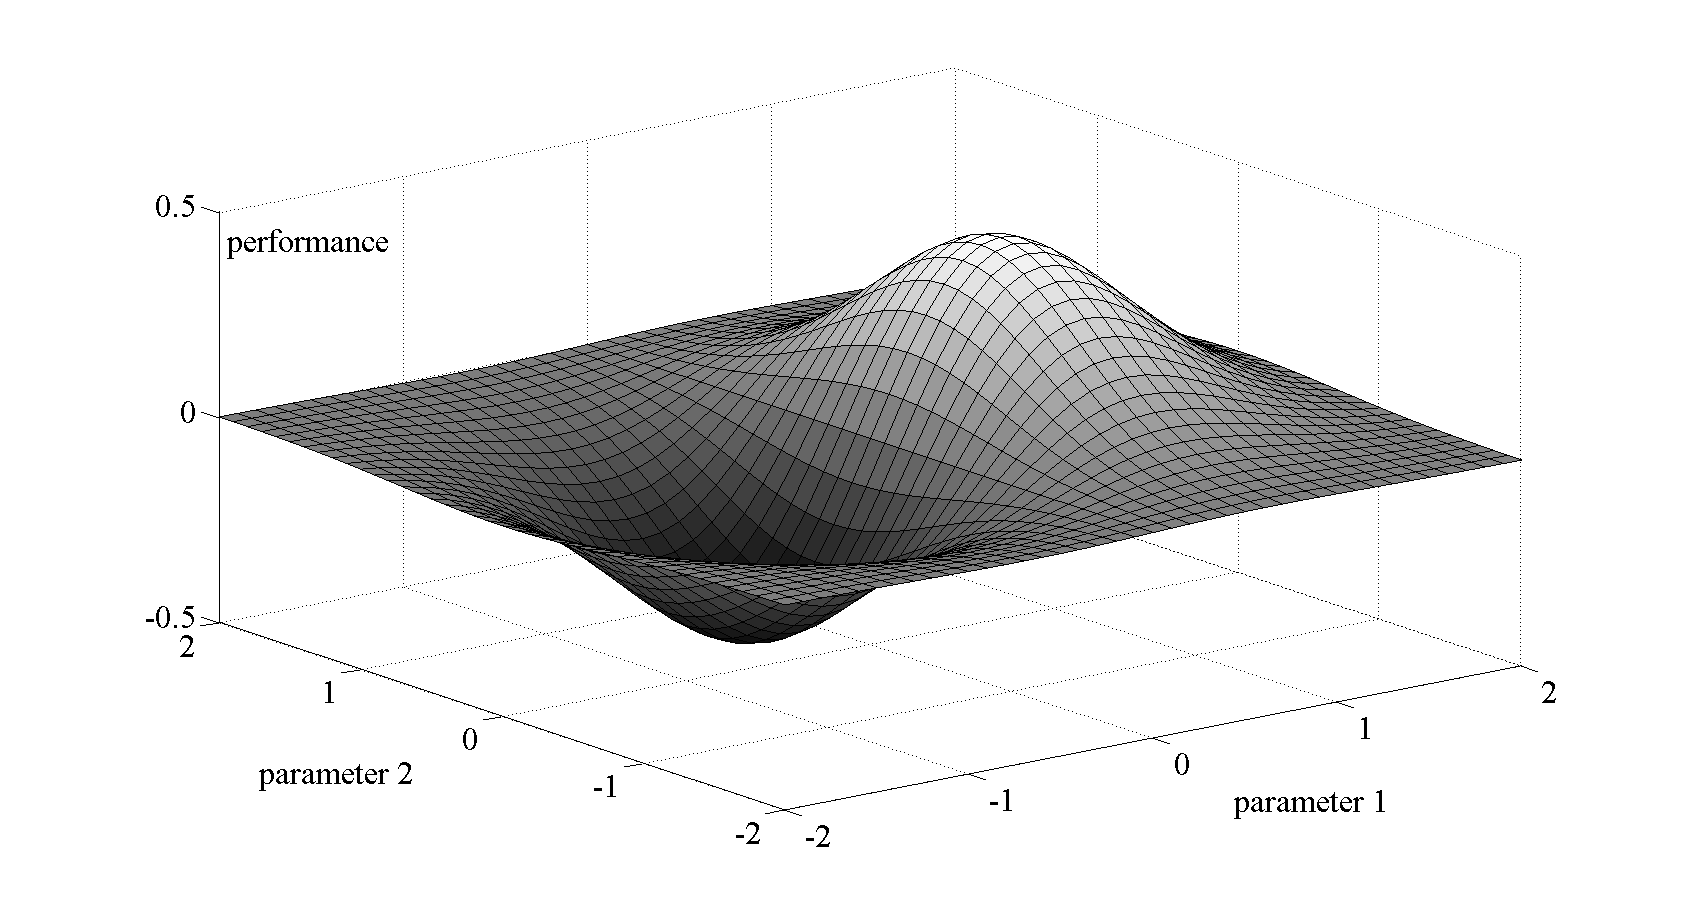
\includegraphics[width=1.0\textwidth]{training_strategy/performance_function.png}
\caption{Geometrical representation of the performance function.}\label{PerformanceFunctionFigure}
\end{center}
\end{figure}

The minimum or maximum value of the performance functional is
achieved for a vector of parameters at which the performance
function takes on a minimum or maximum value. Therefore, the
learning problem for neural networks, formulated as a
variational problem, can be reduced to a function optimization
problem \cite{Lopez2006ICANN}.

In this sense, a variational formulation for neural networks provides a direct method for solving variational 
problems. The universal approximation 
properties for the multilayer perceptron cause neural computation to
be a very appropriate paradigm for the solution of these problems.

\subsubsection{One-dimensional optimization}
\index{one dimensional optimization} 
\index{line search|see{one dimensional optimization}}

\index{relative minimum}
\index{local minimum}

\index{relative maximum}
\index{local maximum}

\index{absolute minimum}
\index{global minimum}

\index{absolute maximum}
\index{global maximum}

\index{first training rate}

Although the performance function is multidimensional, one-dimensional optimization methods are of great importance. 
Indeed, one-dimensional optimization algorithms are very often used inside multidimensional optimization algorithms. 

A function is said to have a relative or local minimum at some point if the function is always greater within some neighbourhood of that point. 
Similarly, a point is called a relative or local maximum if the function is always lesser within some neighbourhood of that point. 

The function is said to have a global or absolute minimum at some point if the function is always greater within the whole domain. 
Similarly, a point will be a global maximum if the function is always greater within the whole domain. 
Finding a global optimum is, in general, a very difficult problem \cite{Wolpert1997}. 

On the other hand, the tasks of maximization and minimization are trivially related to
each other, since maximization of a function is
equivalent to minimization of its negative, and vice
versa.

In this regard, a one-dimensional optimization problem is one in which the argument which minimizes the performance function is to be found. 

The necessary condition states that if the directional performance function has a relative optimum  and if the derivative exists as a finite number. 
The condition for the optimum to be a minimum is that the second derivative is greater than zero, and vice versa. 

The most elementary approach for one-dimensional optimization problems is to use a fixed step size or training rate. 
More sophisticated algorithms which are are widely used are the golden section method and the
Brent's method. Both of the two later algortims begin by bracketing a minimum. 

%\subsubsection{Fixed training rate}
%\index{fixed training rate}
%\index{fixed step size|see fixed training rate}

%The most elementary approach for such a problem is to use a fixed step size, or training rate, and move
%from an initial guess point in a favorable direction (positive or negative). The step size
%used must be small in relation to the final accuracy desired. Although this method is
%very simple to implement, it is not efficient in many cases.

The golden section method brackets that minimum until the distance
between the two outer points in the bracket is less than a defined
tolerance \cite{Press2002}.

The Brent's method performs a parabolic
interpolation until the distance between the two outer points
defining the parabola is less than a tolerance \cite{Press2002}.


\subsubsection{Multi-dimensional optimization}

\index{function optimization problem}
\index{performance function}
\index{global minimum, performance function}
\index{local minimum, performance function}

\index{global minimum condition}
\index{local minimum condition}

\index{epoch}
\index{iteration|see{epoch}}

\index{parameters increment}
\index{training direction}
\index{training rate}

\index{evaluation improvement}

\index{stopping criteria}

\index{minimum parameters increment norm}

\index{evaluation goal}
\index{minimum evaluation improvement}
\index{gradient norm goal}

\index{maximum time}
\index{maximum epochs number}

\index{early stopping}

\index{zero order method}
\index{random search}
\index{evolutionary algorithm}
\index{genetic algorithm|see{evolutionary algorithm}}

\index{first order method}
\index{gradient descent method}
\index{conjugate gradient method}
\index{scaled conjugate gradient}
\index{quasi-Newton method} 

\index{second order method}
\index{Newton's method}
\index{Levenberg-Marquardt algorithm}

As it was shown in Chapter \ref{PerformanceFunctional}, the learning problem for neural networks is reduced 
to the searching for a parameter vector at which the performance function takes
a maximum or a minimum value.

The concepts of relative or local and absolute or global optima for the multidimensional case apply in the same way as for the one-dimensional case. The tasks of maximization and minimization are also trivially related here. 

The necessary condition states that if the neural network is at a minimum of the performance function, 
then the gradient is the zero vector. 

The performance function is, in general, a non linear function of the
parameters. As a consequence, it is not possible to find closed
training algorithms for the minima. Instead, we consider a search
through the parameter space consisting of a succession of steps, or
epochs. 

At each epoch, the performance will increase by adjusting the neural network parameters. 
The change of parameters between two epochs is called the parameters increment. 

In this way, to train a neural network we start with some parameters vector 
(often chosen at random) and we generate a sequence of parameter vectors, so
that the performance function is reduced at each iteration of the algorithm. 
The change of performance between two epochs is called the performance improvement. 

The training algorithm stops when a specified condition is satisfied. 
Some stopping criteria commonly used are \cite{Demuth2009}:

\begin{enumerate}
\item The parameters increment norm is less than a minimum value. 
\item The performance improvement in one epoch is less than a set value.
\item Performance has been minimized to a goal value.
\item The norm of the performance function gradient falls below a goal.
\item A maximum number of epochs is reached.
\item A maximum amount of computing time has been exceeded.
\end{enumerate}

A stopping criterium of different nature is early stopping. 
This method is used in ill-possed problems in order to control the effective complexity of the neural network. 
Early stopping is a very common practice in neural networks and often produces good solutions to ill-possed problems. 

Figure \ref{TrainingProcess} is a state diagram of the training
procedure, showing states and transitions in the training process
of a neural network.

\begin{figure}[h!]
\begin{center}
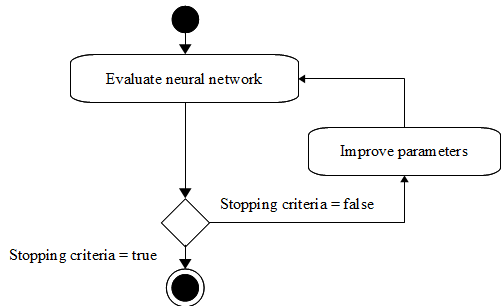
\includegraphics[width=0.8\textwidth]{training_strategy/training_process.png}
\caption{Training process.}\label{TrainingProcess}
\end{center}
\end{figure}

The training process is determined by the way in which the
adjustment of the parameters in the neural network takes place.
There are many different training algorithms, which have a variety
of different computation and storage requirements. Moreover, there
is not a training algorithm best suited to all locations
\cite{Wolpert1997}.

Training algorithms might require information from the performance
function only, the gradient vector of the performance function or the
Hessian matrix of the performance function \cite{Press2002}. These
methods, in turn, can perform either global or local optimization.

Zero-order training algorithms make use of the performance function
only. The most significant zero-order
training algorithms are stochastic, which involve randomness in the
optimization process. Examples of these are random
search and evolutionary
algorithms \cite{Goldberg1988}
\cite{Fogel1994} or particle swarm optimization \cite{Kennedy1995},
which are global optimization methods .

First-order training algorithms use the performance function and its
gradient vector \cite{Battiti1992}.
Examples of these are gradient descent methods, conjugate gradient methods, scaled conjugate gradient methods \cite{Moller1993} or quasi-Newton
methods. Gradient descent, conjugate
gradient, scaled conjugate gradient and quasi-Newton methods are
local optimization methods \cite{Luenberger1984}.

Second-order training algorithms make use of the performance function,
its gradient vector and its Hessian matrix \cite{Battiti1992}. Examples for second-order methods are
Newton's method and the Levenberg-Marquardt
algorithm \cite{Hagan1994}.
Both of them are local optimization methods \cite{Luenberger1984}.

\subsubsection{Training strategy}

Most of the times, application of a single training algorithm is enough to properly train a neural network. 
The quasi-Newton method is in general a good choice, since it provides good training times and deals successfully with most of the performance functions. 
The Levenberg-Marquardt algorithm could be also recommended for small and medium-sized data modelling problems. 
 
However, some applications might need more training effort. 
In that cases we can combine different algorithms in order to do our best. 
In problems defined by mathematical models, with constraints, etc. a single training algorithm might fail. 

Therefore, for difficult problems, we can try two use two or three different training algorithms. 
A general strategy consists on applying three different training algorithms: 

\begin{enumerate}
\item Initialization training algorithm. 
\item Main training algorithm. 
\item Refinement training algorithm. 
\end{enumerate}

The initialization training algorithm is used to bring the neural network to a stable region of the performance function.
Near the optimum, the performance function usually behaves better than far away. 
Zero order training algorithms, such as random search or the evolutionary algorithm might good for this initialization process. 
Indeed, they are very robust algorithms. 

The main training algorithm does most of the job. The training strategy relies on them. 
First order training algorithms, such as the quasi-Newton method are a good choce here. 

Finally, a refinement training algorithm can be used when a big accuracy is required. 
Second orden training algorithms, such as the Newton-method, require the most exact information of the performance function. Therefore they can perform better for refinement. 

